\documentclass[10pt]{article}
\usepackage{icmlko}

\icmlmeta{IP 파운데이션 월드모델}{246}{남이 치른다}{모바일 가격 눈금을 고치면 값은 모바일에서만 바뀌는데 판은 웹툰에서 무너진다 --- 손해의 96\%가 자료를 안 건드린 도메인에서 나온다}

\begin{document}

\twocolumn[
\icmlheader

\begin{abstract}
노트 245가 ``$|\Delta| \le 0.010$ 자리는 다투지 말라''는 규약을 남겼으니,
0.010 위를 골랐다. 노트 243이 잰 축별 무게에서 제일 무거운 것은
\texttt{entry\_friction} 이다 --- 빼면 $-$0.0637 이다. 그리고 노트 240이 그
축에 진짜 버그가 있다고 적어 뒀다: \texttt{mobile\_axes.py} 의
\texttt{scale01(price, 0, 15)} 는 \emph{달러}로 쓴 경계인데 값은 \emph{원}이라
1,100원부터 44,000원까지 유료 709건(35.4\%)이 전부 1.0 으로 뭉개진다.
\textbf{서로 다른 값이 둘뿐인 무료/유료 깃발}이다. 노트 240은 넷을 한꺼번에
고쳐 $-$0.0332 를 봤는데, 이번엔 \textbf{모바일 하나만} 고쳤다. 두 가지 안 ---
경계를 실제 범위로 넓히기, 그리고 노트 240이 ``고원이 정보''라고 한 것을
살려 무료는 0 으로 두고 유료 안에서만 등급을 매기기. \textbf{둘 다 크게
진다}($-$0.0377 · $-$0.0336). 누가 치르는지 갈랐더니 답이 이상하다 ---
\textbf{모바일이 낸 몫은 $-$0.0012(3.6\%)이고 나머지 여덟이 $-$0.0320(96\%)를
낸다.} 웹툰이 $-$0.0766, 애니가 $-$0.0441, 아이돌은 $+$0.1542에서
$-$0.1130으로 \textbf{부호가 뒤집힌다}. 자료가 한 글자도 안 바뀐 도메인들이다.
손 축 다섯은 \textbf{공유 계수}를 쓰므로, 한 도메인의 눈금을 고치는 것은
국소 결정이 아니다. 제대로 된 길 --- 모바일에게 \texttt{entry\_friction}
전용 기울기를 주는 것 --- 은 노트 241이 이미 막아 뒀다($-$0.0309). \textbf{두
길이 다 막혔으므로 값 둘짜리 깃발을 그대로 둔다.} 국소적으로는 열등한
부호화가 전역적으로는 최적이다.
\end{abstract}
]

\section{0.010 위를 골랐다}

노트 245의 규약은 소극적이다 --- 작은 자리는 안쪽으로도 유보로도 못 정하니
다투지 않는다. 그러면 무엇을 다투나. 노트 243이 축을 하나씩 빼서 만든 표가
그대로 답이다. 제일 무거운 축은 \texttt{entry\_friction} 이다.

\begin{center}\small
\begin{tabular}{lr}
\hline
축 & 빼면 \\
\hline
\texttt{entry\_friction} & $-$0.0637 \\
\texttt{target\_breadth} & $-$0.0304 \\
\texttt{media\_push} & $-$0.0150 \\
\texttt{goods\_scale} & $-$0.0131 \\
\texttt{trend\_momentum} & $-$0.0094 \\
\hline
\end{tabular}
\end{center}

그리고 그 축에는 노트 240이 찾아 둔 진짜 버그가 있다.

\section{값이 둘뿐인 축}

\begin{quote}\small
\texttt{mobile\_axes.py:} \\
\texttt{\ a["entry\_friction"] = scale01(float(p), 0.0, 15.0)} \\
\texttt{\ why[...] = f"\{p:.2f\} 달러" if p else "무료"}
\end{quote}

주석은 달러라고 말하는데 값은 원이다(0 · 1,100 · 3,300 · 4,400 · 6,600 ·
7,700 $\dots$ 44,000). 경계가 15 이니 유료는 전부 1.0 이다. \textbf{2,000건이
값 두 개}(0.0 이 64.5\%, 1.0 이 35.4\%)를 갖는다.

노트 240은 이것을 웹툰 · 세계애니 · 만화의 \texttt{target\_breadth} 와
\emph{함께} 고쳐 $-$0.0332 를 봤고, 그때는 ``뭉갬이 정보다''로 읽었다. 넷을
같이 움직였으니 어느 것이 얼마인지는 몰랐다. 이번엔 모바일 하나만 건드렸다.

\begin{center}\small
\begin{tabular}{lrrr}
\hline
 & 값 개수 & F23 판 & 짝 차 \\
\hline
그대로 (깃발) & 2 & 0.4569 & --- \\
경계를 실제 범위로 & 25 & 0.4194 & $-$0.0377 ($t{=}-5.79$) \\
고원 $+$ 유료 안 등급 & 42 & 0.4234 & $-$0.0336 ($t{=}-4.94$) \\
\hline
\end{tabular}
\end{center}

둘째 안은 노트 240의 교훈을 일부러 살린 것이다 --- 무료/유료 고원은 그대로
두고 유료 709건 \emph{안에서만} 순위를 매긴다. 정보를 더하기만 하고 빼지
않는데도 진다.

\section{누가 치르나}

\begin{figure}[t]
\centering
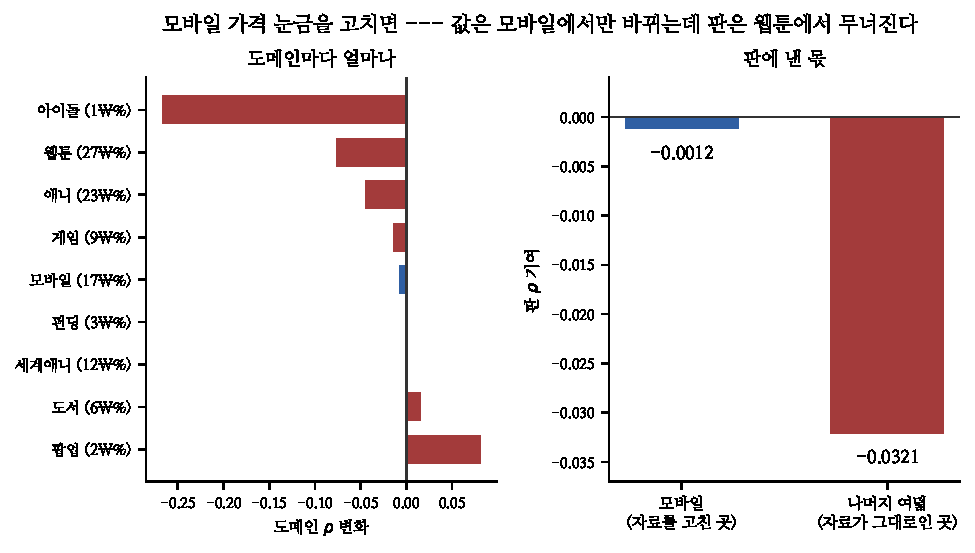
\includegraphics[width=\columnwidth]{figs/whopays.pdf}
\caption{둘째 안(고원 $+$ 등급)에서 도메인마다의 변화와 판 기여.
파랑이 자료를 고친 곳이다.}
\end{figure}

\begin{center}\small
\begin{tabular}{lrrr}
\hline
도메인 & 몫 & $\rho$ 변화 & 판 기여 \\
\hline
웹툰 & 27.3\% & $-$0.0766 & $-$0.0209 \\
애니 & 23.2\% & $-$0.0441 & $-$0.0103 \\
아이돌 & 1.0\% & $\mathbf{-0.2672}$ & $-$0.0026 \\
게임 & 8.6\% & $-$0.0141 & $-$0.0012 \\
\textbf{모바일} & 16.9\% & $\mathbf{-0.0074}$ & $\mathbf{-0.0012}$ \\
세계애니 & 11.5\% & $+$0.0011 & $+$0.0001 \\
도서 & 6.2\% & $+$0.0158 & $+$0.0010 \\
팝업 & 2.3\% & $+$0.0817 & $+$0.0018 \\
\hline
\textbf{모바일} & & & $\mathbf{-0.0012}$ \\
\textbf{나머지 여덟} & & & $\mathbf{-0.0320}$ (96\%) \\
\hline
\end{tabular}
\end{center}

\textbf{자료를 고친 도메인은 거의 안 치르고 안 고친 도메인이 다 치른다.}
아이돌은 $+$0.1542에서 $-$0.1130으로 \textbf{부호가 뒤집힌다} --- 25건짜리
도메인이라 판에는 $-$0.0026 만 내지만, 모바일 가격표를 손봤더니 아이돌
순위가 거꾸로 섰다는 것은 그 자체로 읽어 둘 만하다.

기전은 노트 240에서 이미 봤다. 손 축 다섯은 \textbf{전 도메인이 계수를
공유}한다. 모바일 열의 값이 바뀌면 풀링 능형이 \texttt{entry\_friction}
계수를 다시 맞추고, 그 계수는 웹툰 · 애니 · 아이돌이 같이 쓴다. 노트 240은
새 축을 더해서 이 일을 일으켰고, 여기서는 \textbf{열 하나의 값만} 바꿔
같은 일을 일으켰다 --- 더 깨끗한 시연이다.

\section{두 길이 다 막혔다}

옳은 처방은 뻔해 보인다 --- 모바일에게 \texttt{entry\_friction} 전용
기울기를 주면 좋은 부호화가 남에게 안 샌다. 노트 241이 그것을 이미 쟀다:
\texttt{entry\_friction} 에 도메인별 기울기를 주면 \textbf{$-$0.0309}
($t{=}-5.40$)이다. 손 축 다섯 중 제일 크게 지는 축이 하필 이것이다.

\begin{center}\small
\begin{tabular}{lr}
\hline
길 & 값 \\
\hline
눈금을 고친다 & $-$0.0336 \\
전용 기울기를 준다(노트 241) & $-$0.0309 \\
\textbf{그냥 둔다} & \textbf{0} \\
\hline
\end{tabular}
\end{center}

\textbf{값 둘짜리 깃발을 그대로 둔다.} 모바일만 놓고 보면 열등한 부호화이지만
(모바일 자신도 고치면 $-$0.0074 로 조금 나빠지긴 한다), 판 전체로는 최적이다.
\textbf{국소 최적과 전역 최적이 어긋나는 자리}이고, 어긋나게 만드는 것은
자료가 아니라 \emph{계수를 공유한다는 설계}다.

\paragraph{남은 것}
\begin{center}\small
\begin{tabular}{ll}
\hline
갈래 & 왜 \\
\hline
공유 계수 & 손 축 다섯이 다 이렇다. 구조를 바꿀 길이 있나 \\
아이돌 부호 뒤집힘 & 25건이 남의 눈금에 이만큼 흔들린다 \\
\texttt{target\_breadth} & 두 번째로 무거운 축($-$0.0304). 여기도 그런가 \\
0.010 위 목록 & 노트 243 표에 다섯 줄뿐이다. 더 있나 \\
\hline
\end{tabular}
\end{center}

\paragraph{규약} \textbf{한 도메인의 축 값을 고치는 것은 국소 결정이 아니다.}
고치기 전에 그 축이 공유 계수인지 보고, 공유라면 \emph{안 고친 도메인들}에서
재라. 이번 경우 모바일만 봤으면 $-$0.0074 짜리 작은 손해로 보였을 것이고,
그건 노트 245의 규약에 따라 ``다투지 않는 자리''로 넘어갔을 것이다.

\end{document}
